%% LaTeX Beamer presentation template (requires beamer package)
%% see http://bitbucket.org/rivanvx/beamer/wiki/Home
%% idea contributed by H. Turgut Uyar
%% template based on a template by Till Tantau
%% this template is still evolving - it might differ in future releases!

\documentclass[brazil]{beamer}

\mode<presentation>
{
\usetheme{LRM}
\setbeamercovered{transparent}
\setbeamertemplate{footline}[page number]
}


\usepackage[brazil]{babel}
\usepackage[utf8]{inputenc}

% font definitions, try \usepackage{ae} instead of the following
% three lines if you don't like this look
\usepackage{mathptmx}
\usepackage[scaled=.90]{helvet}
\usepackage{courier}
\usepackage[T1]{fontenc}


\title[Projeto de Mestrado]{
Navegação de Veículos Autônomos em Ambientes Externos 
Não Estruturados Baseada em Visão Computacional}

\author[Rafael Luiz Klaser]{Rafael Luiz Klaser \\
Orientador: Prof. Dr. Fernando Santos Osório}

\institute[ICMC - USP São Carlos]
{
Laboratório de Robótica Móvel\\

\includegraphics[width=2cm,height=1cm,clip=true]{../img/icmc.png}
}

\date{Abril 2013}

\bibliography{quali}

\begin{document}

\begin{frame}
\titlepage

\includegraphics[width=2cm,height=0.5cm,clip=true]{../img/fapesp.jpg}
\textit{\tiny Apoio \#2012/04555-4}
\end{frame}

\begin{frame}
\frametitle{Sumário}
\framesubtitle{roteiro da apresentação}
\tableofcontents
\end{frame}

\section{Introdução}

\subsection[Motivação]{Motivação}


\begin{frame}
\frametitle{Introdução}
\framesubtitle{Motivação}
\begin{block}{Aplicações}
Os veículos autônomos tem recebido destaque em diversas aplicações onde a
presença de pessoas as coloca em situação de risco, desconforto, fadiga ou
requerem algum tipo de precisão onde a máquina está mais apta a executar determinada
tarefa.
\end{block}
\begin{block}{}
Um exemplo de aplição para veículos terrestres em ambiente não estruturado é
no auxílio ao combates a incêndios florestal. 
\end{block}
\end{frame}


\begin{frame}
\frametitle{Introdução}
\framesubtitle{Motivação - Aplicações}
05/04/2013 - Notícia ClicRBS: 
\textbf{Levantamento indica que cerca de 5.000 hectares foram queimados no
incêndio do Taim}
O incêndio no Taim começou no dia 26 de março e demorou 9 dias para ser
controlado
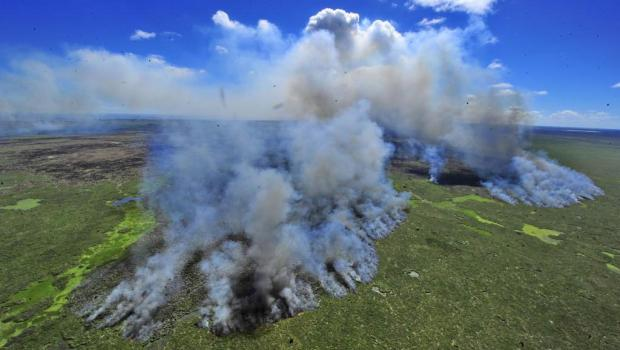
\includegraphics[width=8cm,height=4cm,]{../img/14817864.jpg}
\\Foto: Lauro Alves  / Agência RBS
\end{frame}


\begin{frame}
\frametitle{Introdução}
\framesubtitle{Motivação}
\begin{itemize}
  \item Os veículos autônomos tem tido destaque na comunidade
científica pelos seus desafios e potencial de aplicação junto à
sociedade – atualmente os estudos relacionados a esta área
tem aumentado significativamente;
  \item A Visão Computacional é uma área com diversos problemas
em aberto (O próprio funcionamento da visão biológica é
ainda pouco conhecido);
  \item Este projeto de pesquisa tem por base o trabalho “Robôs-
Bombeiros” de Gustavo Pessin (Evolução de estratégias e controle
inteligente em sistemas multi-robóticos robustos. Dissertação de
Mestrado. 2008).
\end{itemize}
\end{frame}

\begin{frame}
\frametitle{Introdução}
\framesubtitle{Trabalhos Relacionados}
ELROB – European Robot Trial
\begin{itemize}
  \item Exibição onde são demonstradas e comparadas as capacidade dos sistemas de
veículos autônomos (no cenário “off-road”);
  \item Ocorre a anualmente, intercalando entre objetivo militar e civil a cada
ano. (a próxima exibição civil ocorrerá em 9/2013 – Alemanha);
  \item Projetos europeus
\end{itemize}
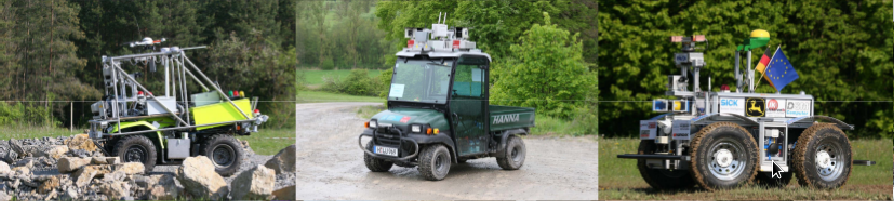
\includegraphics[width=10cm,height=3cm,]{../img/elrob.png}
\end{frame}


\begin{frame}
\frametitle{Introdução}
\framesubtitle{Definição do problema}
\begin{block}{Definição do problema}
Dada uma origem do veículo e um destino (referenciados por GPS) em um terreno
não estruturado com vegetação, navegar de forma autônoma desviando dos
obstáculos e conduzindo o veículo até o destino. 
\end{block}
\end{frame}

\subsection[Objetivo]{Objetivo}

\begin{frame}
\frametitle{Introdução}
\framesubtitle{Objetivo}
\begin{block}{Objetivo}
Desenvolver um método de navegação autônoma, reativo/deliberativo, focado em
ambientes externos não estruturados, com base em um mapa de navegabilidade com informação
espacial (tridimensional) construído a partir de visão estéreo.
\end{block}
\end{frame}

\subsection[Contribuições]{Contribuições esperadas}

\begin{frame}
\frametitle{Introdução}
\framesubtitle{Contribuições}
% Contribuição para a percepção espacial em métodos de navegação autônoma de
% robôs terrestres,
\begin{itemize}
\item Aperfeiçoamento de algoritmos de geração de mapas de disparidade e nuvem de pontos;
\item Proposta e desenvolvimento de algoritmo para a obtenção de mapas locais de 
navegabilidade com informações espaciais (3D);
\item Aperfeiçoamento de técnicas para a navegação baseada no uso de GPS, 
bússola e mapas locais de navegabilidade (onde as pesquisas previamente 
desenvolvidas para detectar e desviar de obstáculos com o uso de mapas 2D 
serão estendidas a fim de trabalhar com mapa de navegabilidade/ocupação em 3D).
\end{itemize}
\end{frame}


\subsection[Conceitos]{Conceitos abordados}

\begin{frame}
\frametitle{Introdução}
\framesubtitle{Conceitos abordados}
\begin{itemize}
\item Visão estéreo / Calibragem;
\item Mapas de disparidade;
\item Nuvens de pontos;
\item Representação espacial;
\item Mapa de navegabilidade.
% \item Navegação
\end{itemize}
\end{frame}

%\subsection[Conceitos]{Visão Computacional}

\begin{frame}
\frametitle{Introdução}
\framesubtitle{Visão Computacional}
\begin{itemize}
  \item Extrair e processar informações a partir de imagens:
  \begin{itemize}
    \item Grande quantidade de métodos e algoritmos;
    \item É comum encontrar diversas restrições (luminosidade, sombras,
    resolução).
  \end{itemize}
  \item O elevado custo computacional de alguns métodos os tornam inviáveis
  quando há a necessidade de execução em tempo real – caso da robótica;
  \item Porém, com o aumento da capacidade dos computadores atuais, o número de
  trabalhos em visão estéreo cresceu significativamente (GPU).
\end{itemize}
\end{frame}

\begin{frame}
\frametitle{Introdução}
\framesubtitle{Visão Computacional}
\begin{itemize}
  \item A calibração é um passo importante quando se lida com câmeras (em visão estéreo é essencial)
   \begin{itemize}
     \item É necessário retificar as distorções provocadas pelas lentes;
     \item Os parâmetros do modelo de projeção (perspectiva) são essenciais para
     a reconstrução tridimensional;
     \item Uma boa calibração pode definir o “sucesso” do método.
\end{itemize}
\end{itemize}
\end{frame}


\begin{frame}
\frametitle{Introdução}
\framesubtitle{Mapa de disparidade}

\begin{itemize}
  \item O mapa de disparidade pode ser construído a partir de duas poses
  deslocadas da mesma cena, com a triangulação de cada ponto com a sua projeção em cada imagem é possível
  estimar a profundidade relativa dos pontos;
  \item O grande problema é determinar qual ponto em uma imagem corresponde ao
  mesmo ponto na outra imagem.
  \item Existem diversas abordagens para tratar esse problema. O \textit{Block
  Matching} é muito utilizado por ser rápido porém é sensível a uma boa
  parametrização (ex. tamanho do bloco de busca).
\end{itemize}

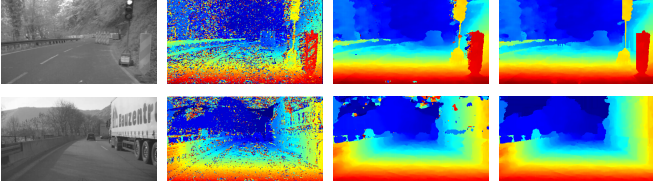
\includegraphics[width=10cm,height=3cm,]{../img/disp_map.png}

%Trabalho recente propondo melhorias: Zhang, Z. et.al - Local stereo
%disparity estimation with novel cost aggregation for sub-pixel accuracy
%improvement in automotive applications, Intelligent Vehicles
%Symposium (IV), 2012 IEEE.

\end{frame}


\begin{frame}
\frametitle{Introdução}
\framesubtitle{Nuvem de pontos}

\begin{itemize}
  \item Localização tridimensional (métrica) dos pontos da imagem obtido a
  partir do mapa de disparidade;
  \item O cálculo das coordenadas é feito utilizando os parametros de calibração
  (distância focal, distância entre as câmeras)
  \item Geralmente se ignora os pontos a uma determinada distância pois o erro
  de posição cresce com disparidades baixas;
  \item A partir de imagens são geradas nuvens densas.
\end{itemize}
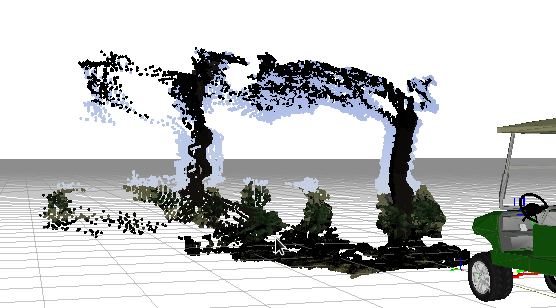
\includegraphics[width=10cm,height=3cm,]{../img/point_cloud_3b.png}

\end{frame}

\begin{frame}
\frametitle{Introdução}
\framesubtitle{Nuvem de pontos}
Exemplo
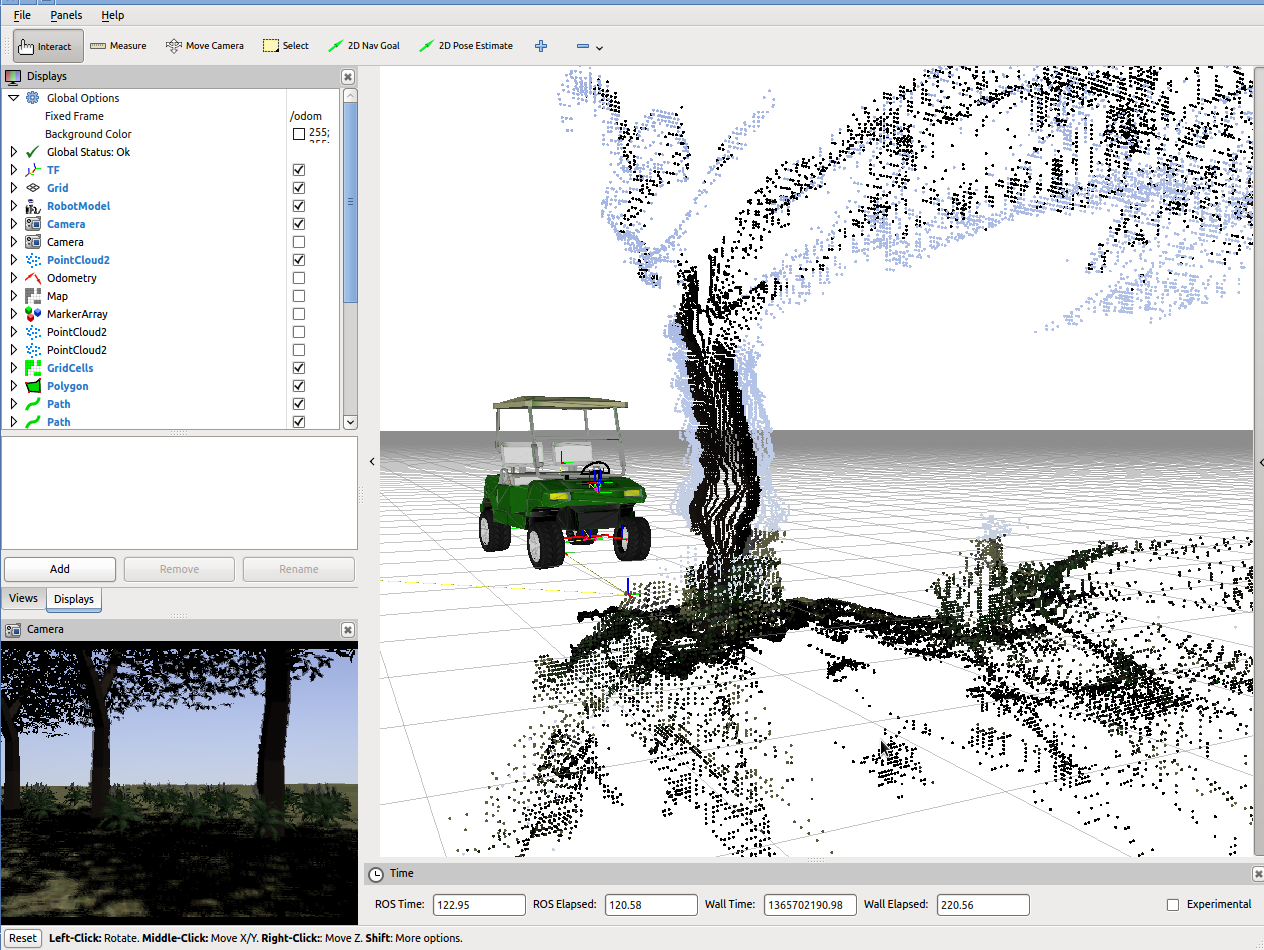
\includegraphics[width=10cm,height=7cm,]{../img/point_cloud_4.png}
\end{frame}


\begin{frame}
\frametitle{Introdução}
\framesubtitle{Representação Espacial}
\begin{itemize}
  \item Uma forma de representar a informação tridimensional de forma
  estruturada é utilizando o conceito de \textit{octree}.
  \item A \textit{octree} é uma árvore que representa o espaço discretizado em
  subdivisões cúbicas;
  \item Desta forma é possível percorrer os dados espaciais de forma
  estruturada;
 \end{itemize}
\center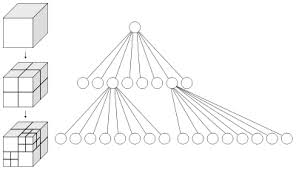
\includegraphics[width=7cm,height=4cm,]{../img/octree.jpg}
\end{frame}

\begin{frame}
\frametitle{Introdução}
\framesubtitle{Representação Espacial}
Exemplo
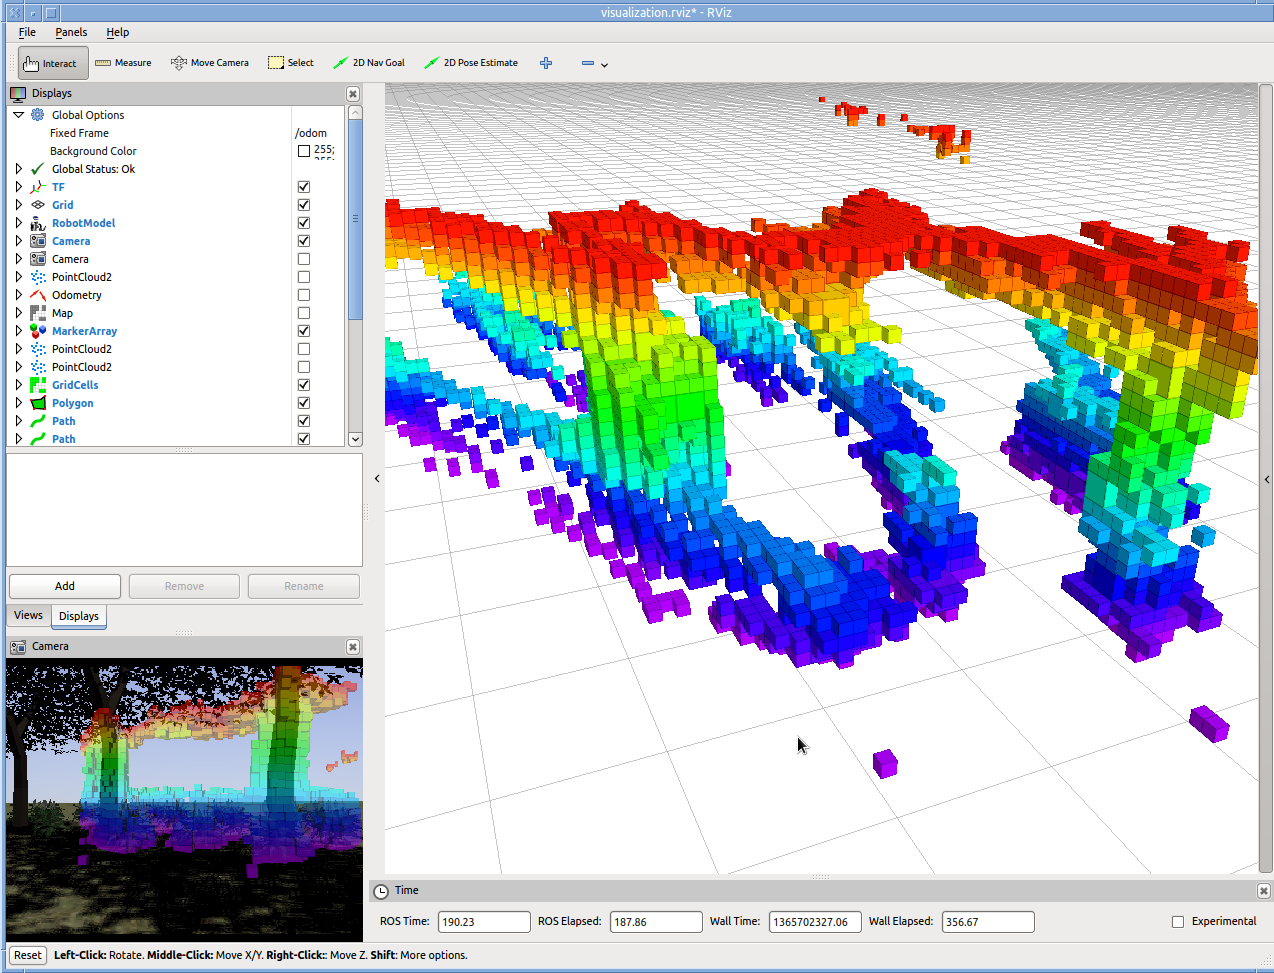
\includegraphics[width=10cm,height=7cm,]{../img/octree_map_2.png}
\end{frame}

\begin{frame}
\frametitle{Introdução}
\framesubtitle{Mapa de navegabilidade}
\begin{itemize}
  \item Representação do terreno navegável, obstruído e desconhecido;
  \item Também é uma representação discretizada do espaço de navegação;
  \item O planejamento de trajetória é efetuado sobre esse mapa;
  \item Um mapa global com informações conhecidas do ambiente pode ser fornecido
  previamente;
  \item Um mapa local é contruído a medida que se explora o ambiente e pode ser
  utilizado para atualizar o mapa global.
 \end{itemize}
\end{frame}

\begin{frame}
\frametitle{Introdução}
\framesubtitle{Mapa de navegabilidade}
Exemplo
\begin{itemize}
  \item Branco: região livre/navegável;
  \item Preto: região com obstáculo;
  \item Cinza: região desconhecida.
\end{itemize}
%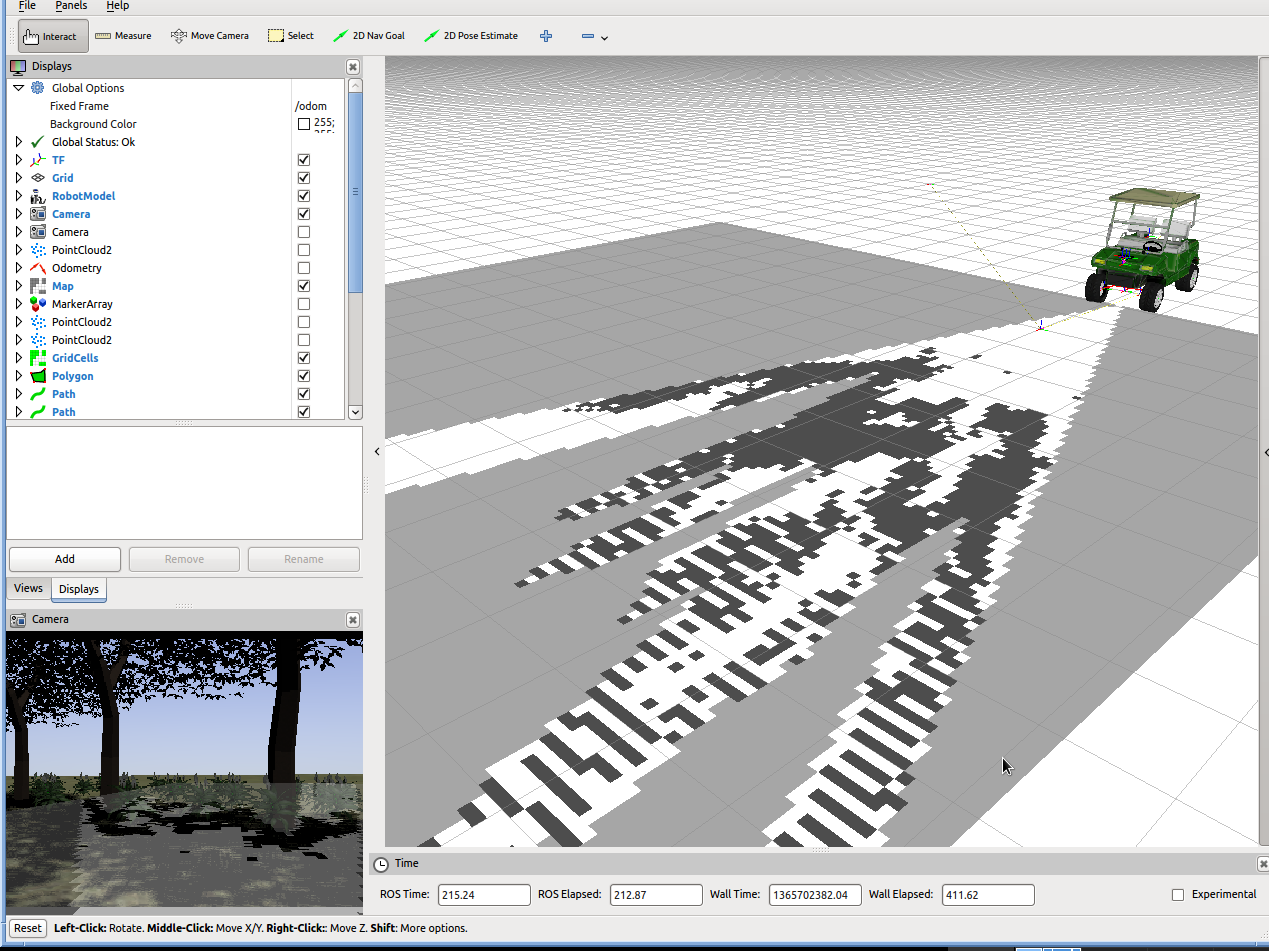
\includegraphics[width=10cm,height=7cm,]{../img/nav_map_1.png}
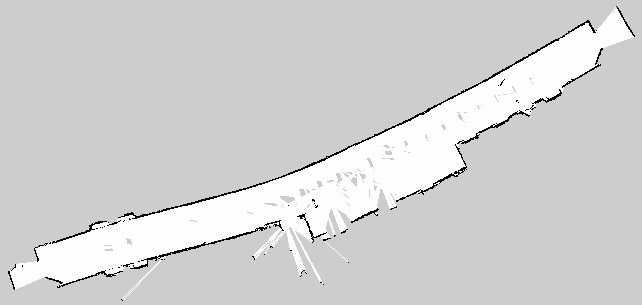
\includegraphics[width=10cm,height=5cm,]{../img/map_2d.jpg}
\end{frame}


\section{Materiais e Métodos}


\begin{frame}
\frametitle{Materiais e Métodos}
\framesubtitle{Equipamentos}
\begin{itemize}
\item Plataforma CaRINA I (veículo)
\item GPS + IMU (localização e odometria)
\item Câmeras de vídeo (binocular, trinocular, etc\ldots)
\end{itemize}
\end{frame}

\begin{frame}
\frametitle{Materiais e Métodos}
\framesubtitle{CaRINA I}
 CaRINA (Carro Robótico Inteligente para Navegação Autônoma)
\begin{columns}[c]
\begin{column}{5cm}
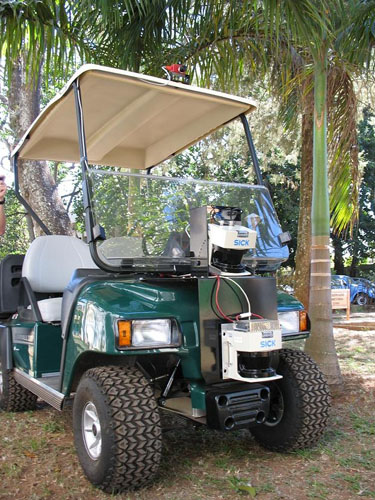
\includegraphics[width=5cm,keepaspectratio]{../img/carina1_1.jpg}
\end{column}
\begin{column}{5cm}
\begin{itemize}
\item 
\includegraphics[width=1.5cm,keepaspectratio]{../img/inct.jpg}
\item 
\includegraphics[width=1.5cm,keepaspectratio]{../img/fapesp.jpg}
\item 
\includegraphics[width=1.5cm,keepaspectratio]{../img/cnpq.png}
\end{itemize}
\end{column}
\end{columns}
\end{frame}

\begin{frame}
\frametitle{Materiais e Métodos}
\framesubtitle{Ferramentas}
\begin{itemize}
\item ROS (Robotic Operating System)
\begin{itemize}
  \item Escolhida por ser amplamente utilizada por grupos de pesquisa em
  robótica;
  \item Plataforma Open-Source
  \item Ferramenta adotada no LRM
\end{itemize}
\item Gazebo - Simulação física (corpos rígidos)
\begin{itemize}
  \item Escolhido por ser um simulador 3D;
  \item Integrado ao ROS
\end{itemize}
\end{itemize}
\end{frame}

\begin{frame}
\frametitle{Materiais e Métodos}
\framesubtitle{ROS}
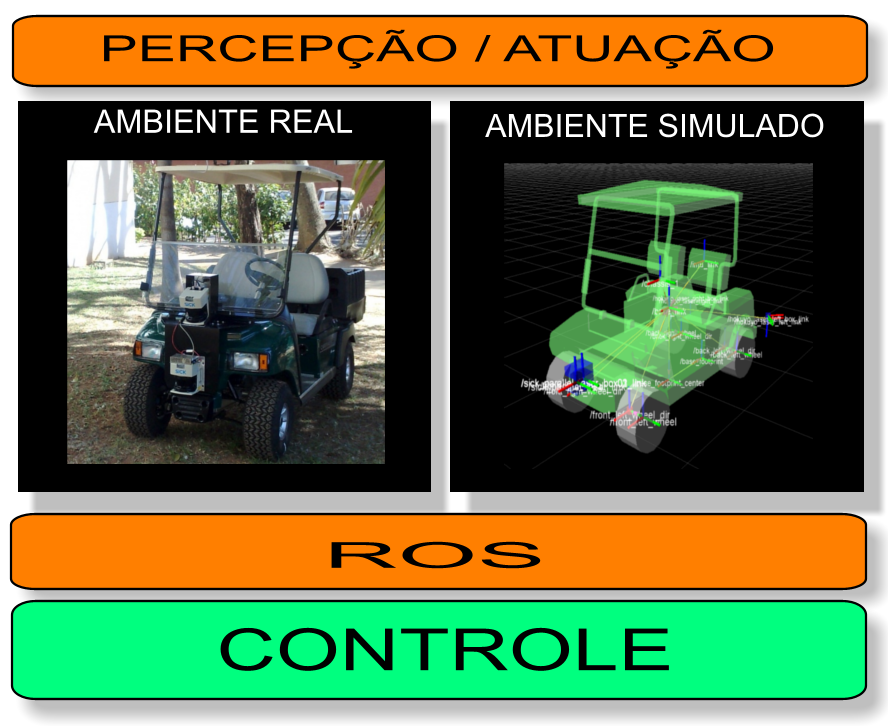
\includegraphics[width=9cm,keepaspectratio]{../img/ros-slide.png}
\end{frame}

%\begin{frame}
%\frametitle{Materiais e Métodos}
%\framesubtitle{ROS}
%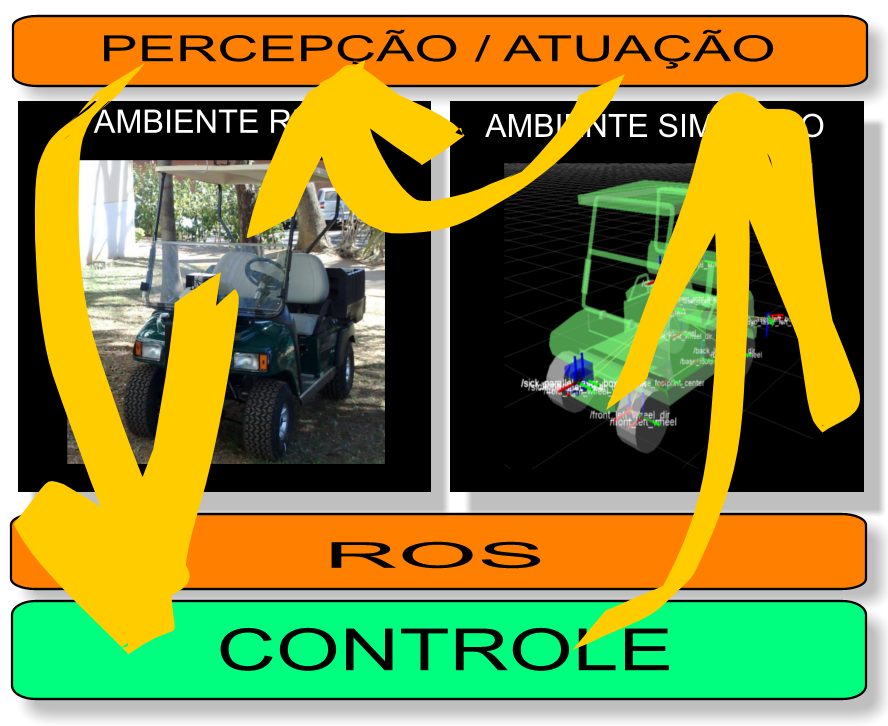
\includegraphics[width=9cm,keepaspectratio]{../img/ciclo-rob.png}
%\end{frame}

%\begin{frame}
%\frametitle{Materiais e Métodos}
%\framesubtitle{ROS}
%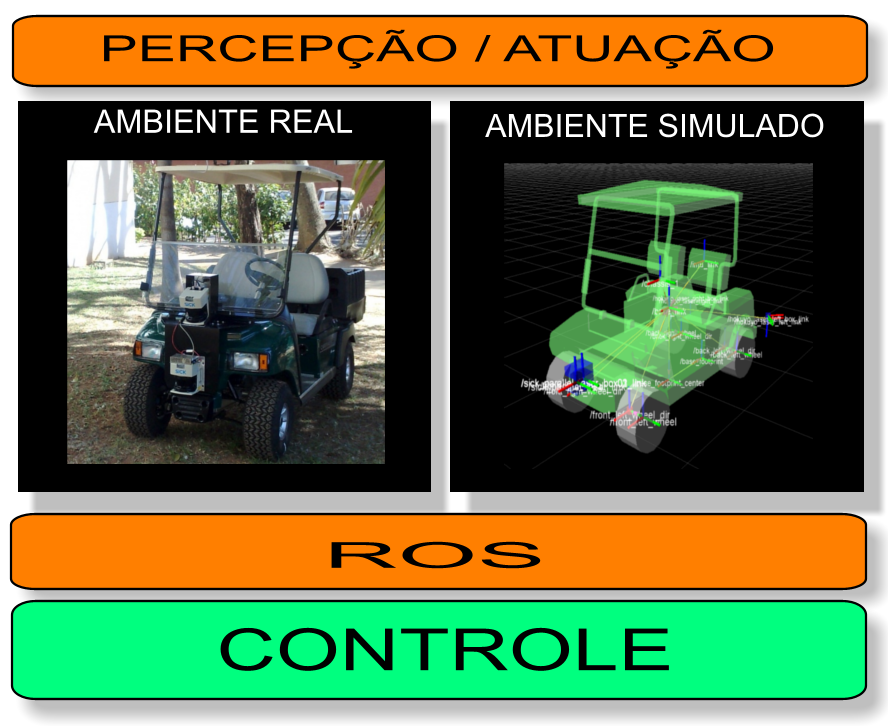
\includegraphics[width=9cm,keepaspectratio]{../img/ros-slide.png}
%\end{frame}

%\begin{frame}
%\frametitle{Materiais e Métodos}
%\framesubtitle{Planejamento}
%\begin{block}{De forma iterativa}
%\begin{block}{}
%\begin{itemize}
%\item Coleta de dados (ambiente real)
%\end{itemize}
%\end{block}
%\begin{block}{}
%\begin{itemize}
%\item Simulação e análise com os dados coletados
%\item Verificação (comportamento) em ambiente simulado 
%\end{itemize}
%\end{block}
%\begin{block}{}
%\begin{itemize}
%\item Validação (ambiente real)
%\end{itemize}
%\end{block}
%\end{block}
%\end{frame}

\begin{frame}
\frametitle{Materiais e Métodos}
\framesubtitle{Simulação}
\begin{block}{Vantagens}
\begin{itemize}
\item Maior repetibilidade dos experimentos
\item Replicação dos experimentos (e sem necessidade do equipamento físico)
\item Versatilidade
\end{itemize}
\end{block}
\begin{block}{Desvantagens}
\begin{itemize}
\item A modelagem dos cenários é custosa (tempo)
\item Não reflete fielmente a realidade
\end{itemize}
\end{block}
\end{frame}

\begin{frame}
\frametitle{Materiais e Métodos}
\framesubtitle{Ambiente Simulado - Gazebo}
Exemplo
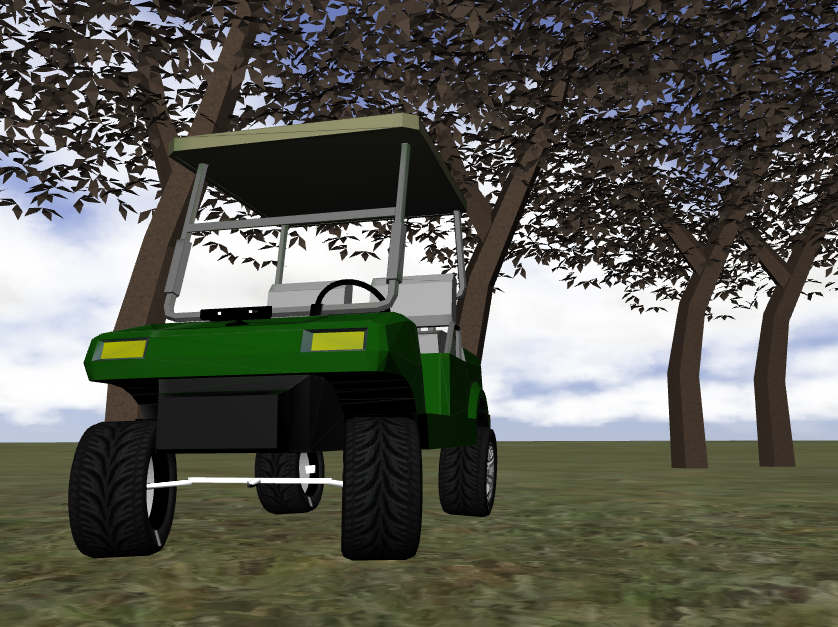
\includegraphics[width=9.5cm,keepaspectratio]{../img/carina_gazebo_frente_fundo.png}
\end{frame}



\section{Proposta de Pesquisa}

\subsection[Tema]{Tema}

%\begin{frame}
%\frametitle{Proposta de Pesquisa}
%\framesubtitle{Temas centrais}
%\begin{itemize}
%\item Visão estéreo
%\item Mapas de navegabilidade a partir de informação tridimensional
%\end{itemize}
%\end{frame}


%\begin{frame}
%\frametitle{Proposta de Pesquisa}
%\framesubtitle{Temas centrais - Propósitos}
%\begin{block}{Visão estéreo}
%Obter a informação espacial do ambiente
%\end{block}
%\end{frame}

%\begin{frame}
%\frametitle{Proposta de Pesquisa}
%\framesubtitle{Temas centrais - Propósitos}
%\begin{block}{Mapa de navegabilidade}
%Para uma navegação deliberativa é necessário o planejamento da trajetória, para
% isso é necessário um mapa (local / global)
%\end{block}
%\end{frame}

\begin{frame}
\frametitle{Proposta de Pesquisa}
\framesubtitle{Temas centrais - Propósitos}

\begin{block}{Visão estéreo}
Obter a informação espacial do ambiente
\end{block}

\begin{block}{Mapa de navegabilidade}
Para uma navegação deliberativa é necessário o planejamento da trajetória, para isso é necessário 
um mapa (local / global)
\end{block}

\end{frame}

%\begin{frame}
%\frametitle{Proposta de Pesquisa}
%\framesubtitle{Planejamento de trajetória\ldots}
%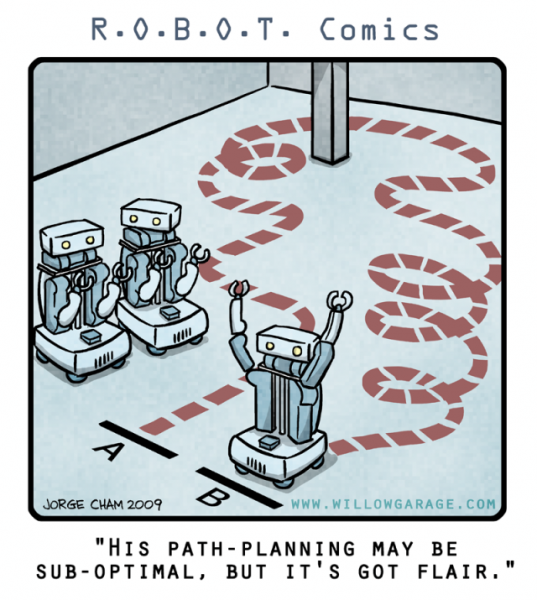
\includegraphics[width=10cm,height=7cm,]{../img/nav_comic.png}
%\end{frame}

\subsection[Discussão]{Discussão}

\begin{frame}
\frametitle{Proposta de Pesquisa}
\framesubtitle{Discussão - Visão Computacional}
\begin{block}{}
Apesar de uma das vantagens das câmeras de vídeo ser a geração de nuvens de pontos densas, 
uma abordagem que produza nuvens menos densas por quadro pode ser aplicada, tendo a densidade 
compensada no tempo (aumentando o desempenho geral sem grande perda da informação global);
\end{block}
\begin{block}{}
A informação global requer maior precisão apenas na trajetória a ser seguida, 
podendo ser aplicado conceito de \textit{foco de atenção};
\end{block}
\end{frame}

%\begin{frame}
%\frametitle{Proposta de Pesquisa}
%\framesubtitle{Discussão - Visão Computacional}
%\begin{block}{}
%Na visão computacional pode-se identificar duas linhas de abordagem: 
%a geométrica e a cognitiva;
%\end{block}
%\begin{block}{}
%Abordagens cognitivas (associas a custo computacional elevado) já se tornam
%praticáveis (computação em GPU) 
%\footnote{Teste preliminar com geração de mapa de disparidade a partir do canal 
%Magno-Celular se demonstrou promissor no conceito de mapas com densidade
%% variável pelo foco de atenção} 
%\end{block}
%\end{frame}

\begin{frame}
\frametitle{Proposta de Pesquisa}
\framesubtitle{Em resumo - Visão Computacional}
\begin{block}{}
A proposta é buscar a geração de nuvens de pontos com a densidade nas regiões de maior
interesse na imagem. 
\end{block}
\end{frame}

\begin{frame}
\frametitle{Proposta de Pesquisa}
\framesubtitle{Discussão - Mapa de navegabilidade}
\begin{block}{}
%As abordagens de navegação por mapas planares assumem condições limitadas do ambiente  
%- geralmente ambiente interno e estruturado.
Um veículo terrestre se desloca na sua superfície de suporte (plano do chão), em condições controladas é
possível limitar-se à uma superfície planar.
\end{block}
\begin{block}{}
Para ambientes externos não estruturados existe maior necessidade da noção espacial 
do ambiente principalmente pela irregularidade do terreno, logo, a abordagem por mapas
que contenham essa noção é justificada. 
\end{block}
\end{frame}

\begin{frame}
\frametitle{Proposta de Pesquisa}
\framesubtitle{Discussão - Mapa de navegabilidade}
\begin{block}{}
Será utilizado o conceito de ocupação com probabilidade associada pois permite melhor atualização dos mapas.
%\textit{Porém seria interessante classificar tais regiões e suas 
%probabilidades também com possíveis elementos ``transponíveis'' - Trabalhos
% futuros.}
\end{block}
\begin{block}{}
Uma vegetação não é necessariamente um obstáculo bloqueante, podendo ser transponível (ex grama, capim);
\end{block}
\end{frame}

\begin{frame}
\frametitle{Proposta de Pesquisa}
\framesubtitle{Em resumo - Mapa de navegabilidade}
\begin{block}{}
A proposta é buscar uma representação em mapa suficiente para descrever o espaço de navegação
do veículo.
\end{block}
%\begin{block}{}
%Idealmente seria desejável uma representação semelhante a um mapa topográfico -
% Trabalhos futuros.
%\end{block}
\end{frame}


\section{Resultados Parciais}

\begin{frame}
\frametitle{Resultados parciais}
\framesubtitle{Arquitetura do sistema}
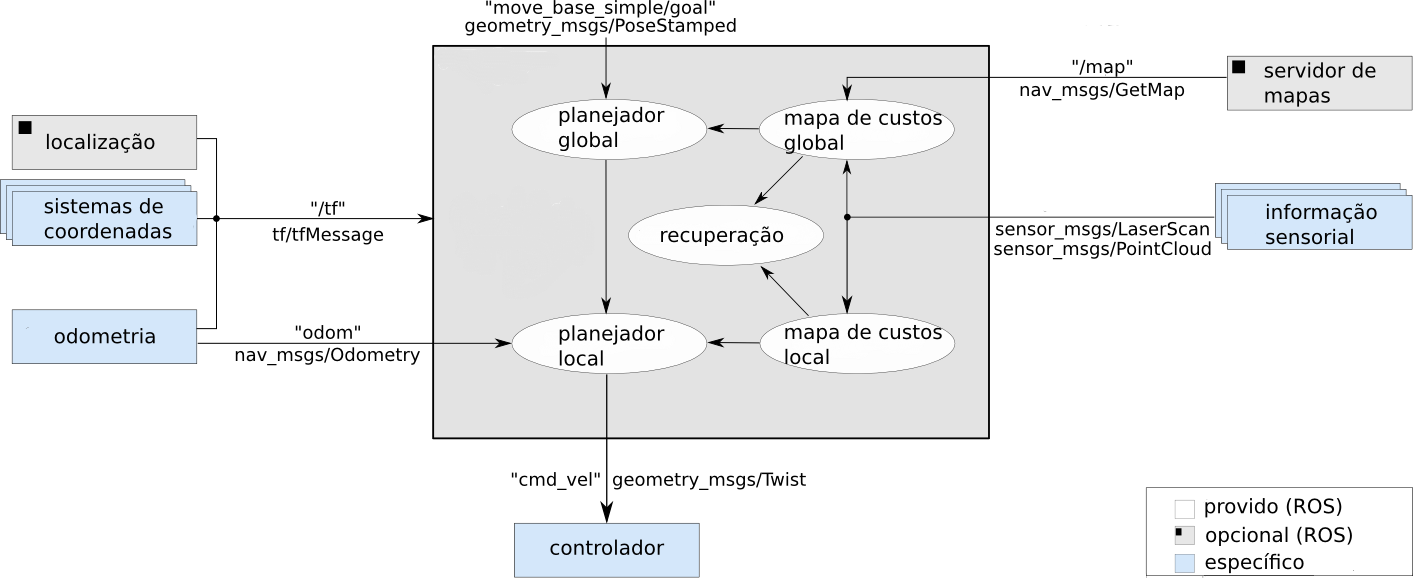
\includegraphics[width=10cm,height=7cm,]{../img/overview_tf_pt.png}
\end{frame}

\begin{frame}
\frametitle{Resultados parciais}
\framesubtitle{Modelagem do veículo}
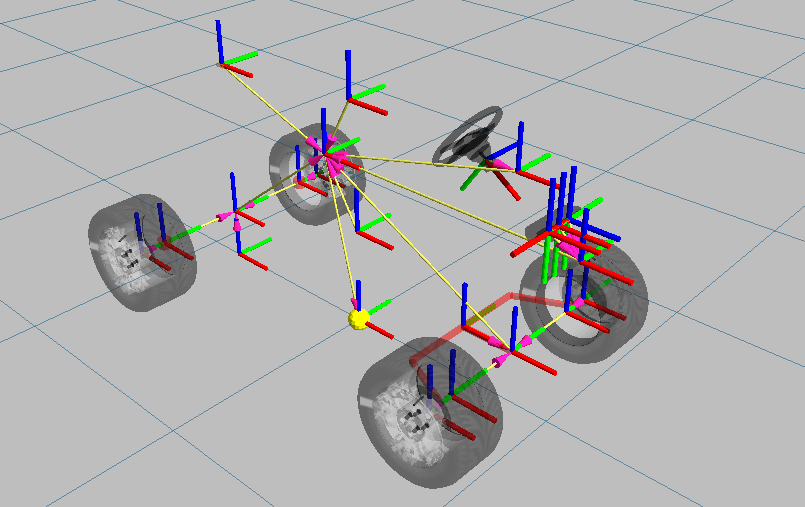
\includegraphics[width=10cm,height=7cm,]{../img/carina_tf_side_wheels_transp.png}
\end{frame}

\begin{frame}
\frametitle{Resultados parciais}
\framesubtitle{Modelagem do veículo}
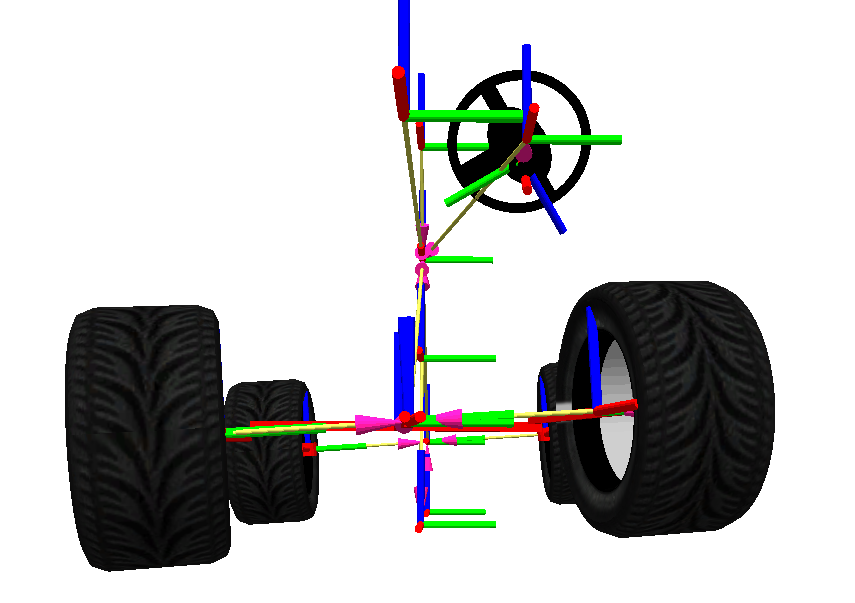
\includegraphics[width=10cm,height=7cm,]{../img/carina_rviz_uneven_susp.png}
\end{frame}


\begin{frame}
\frametitle{Resultados parciais}
\framesubtitle{Odometria e Localização por GPS}
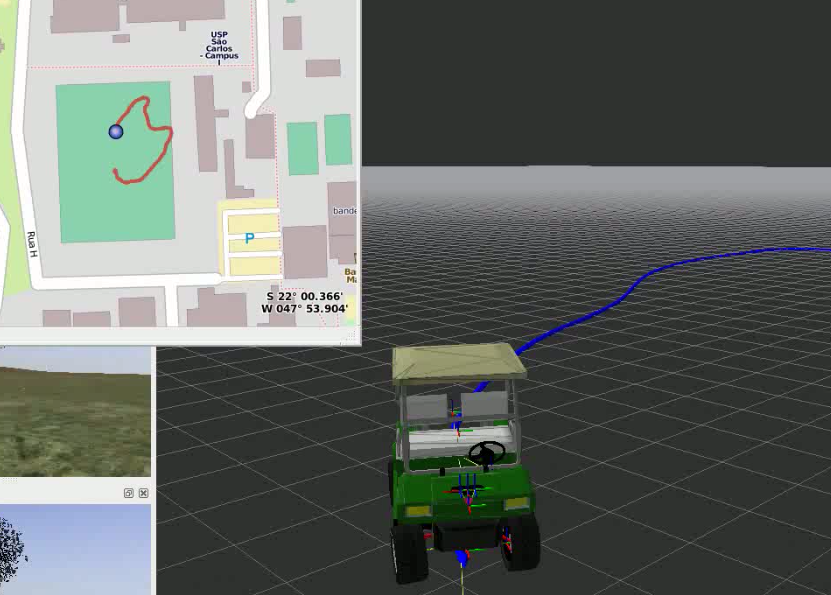
\includegraphics[width=10cm,height=7cm,]{../img/arq_odogps.png}
\end{frame}


\begin{frame}
\frametitle{Resultados parciais}
\framesubtitle{Imagem - Câmera Estéreo}
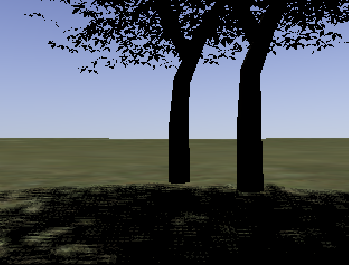
\includegraphics[width=10cm,height=7cm,]{../img/arq_image.png}
\end{frame}

\begin{frame}
\frametitle{Resultados parciais}
\framesubtitle{Cálculo da disparidade}
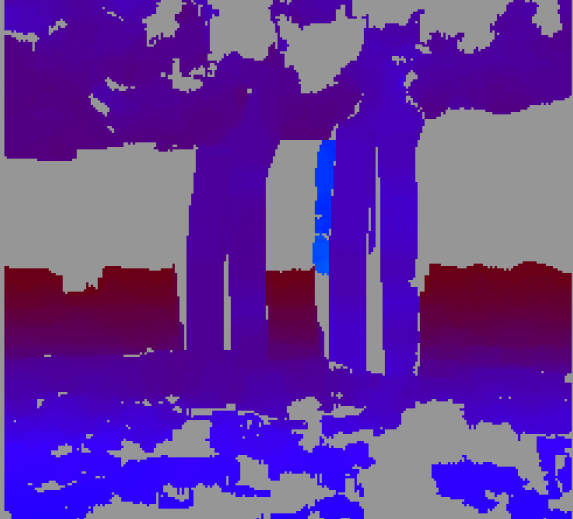
\includegraphics[width=10cm,height=7cm,]{../img/arq_disp.png}
\end{frame}

\begin{frame}
\frametitle{Resultados parciais}
\framesubtitle{Nuvem de pontos}
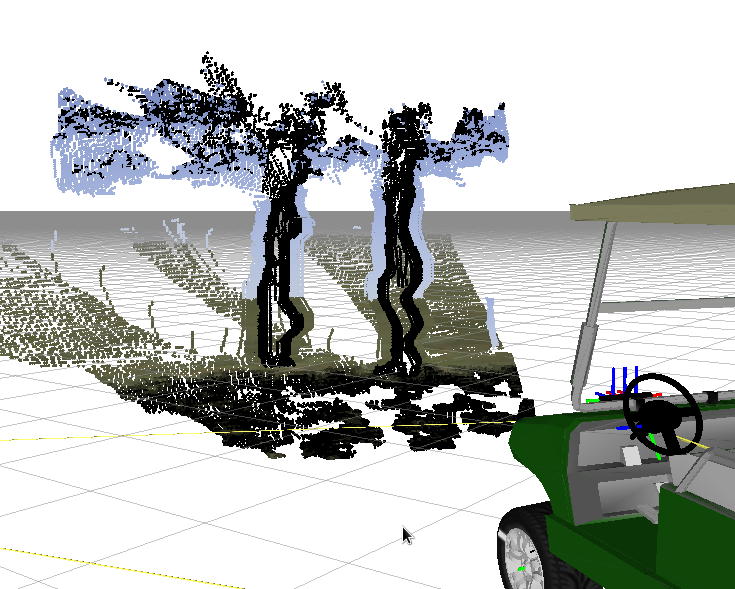
\includegraphics[width=10cm,height=7cm,]{../img/arq_cloud.png}
\end{frame}

\begin{frame}
\frametitle{Resultados parciais}
\framesubtitle{Octomap - Discretização/Agrupamento}
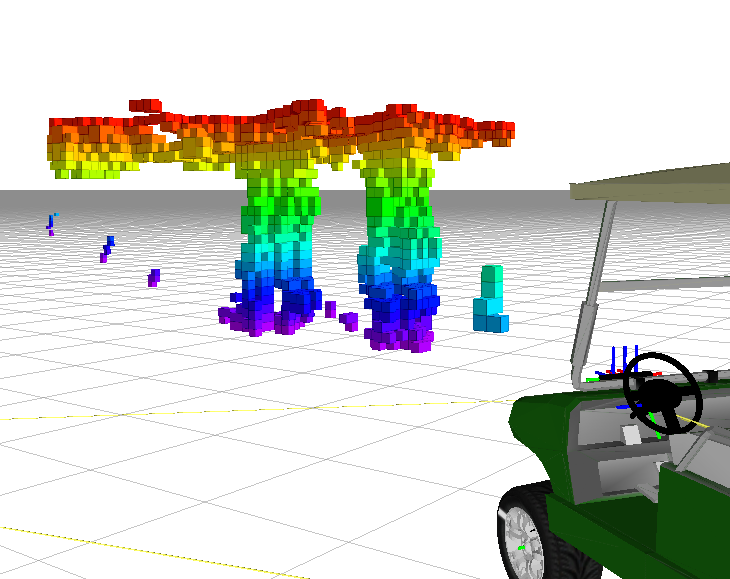
\includegraphics[width=10cm,height=7cm,]{../img/arq_octomap.png}
\end{frame}

\begin{frame}
\frametitle{Resultados parciais}
\framesubtitle{Mapa de Ocupação / Navegabilidade}
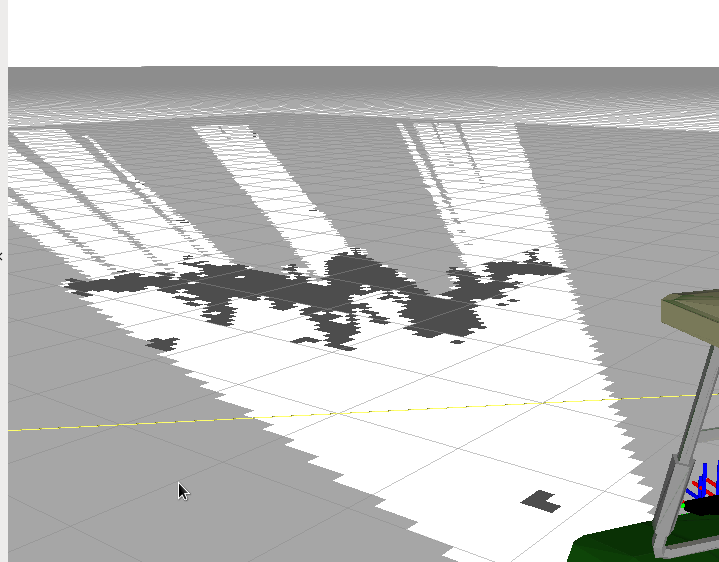
\includegraphics[width=10cm,height=7cm,]{../img/arq_mapa.png}
\end{frame}


\begin{frame}
\frametitle{Resultados parciais}
\framesubtitle{Participação em publicações}
\begin{block}{Dez/2012 : SoCo - Soft Computing}
\textbf{Applying Swarm Intelligence to a Garbage an Recycling Collection
Problem.}\\
\textit{Patrícia A. Vargas; Gustavo Pessin; Daniel O. Sales; Maurício A. Dias; Rafael L. Klaser;
Fernando S. Osório}
\end{block}

\begin{block}{Jan/2013 : JSA - Journal of System Architecture}
\textbf{CaRINA Intelligent Robotic Car: Architectural Design and
Implementations.}\\
\textit{Leandro C. Fernandes; Jeferson R. Souza; Gustavo Pessin; Patrick Y.
Shinzato; Daniel Sales; Caio Mendes; Marcos Prado; Rafael L. Klaser; André Chaves Magalhães; Daniel
Pigatto; Kalinka Castelo Branco; Valdir Grassi Jr.; Fernando S. Osório; Denis F. Wolf,}
\end{block}

\end{frame}




\section{Cronograma}


\framesubtitle{Macro Atividades}
\begin{frame}
\frametitle{Cronograma}
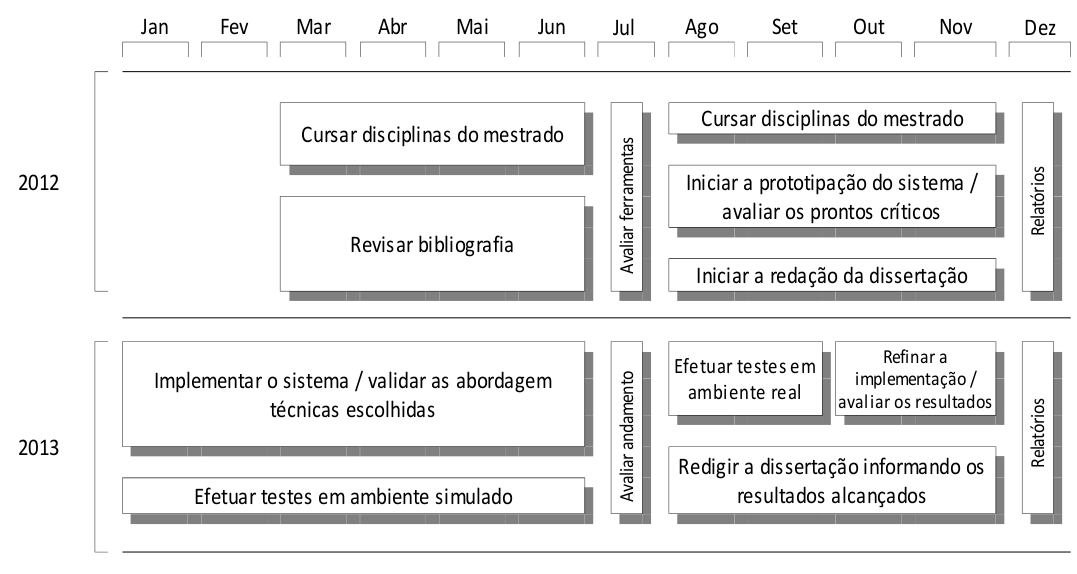
\includegraphics[width=10cm,height=7cm,]{../img/chrono.png}
\end{frame}


\begin{frame}
\frametitle{Perguntas?}
\centering
\begin{columns}[t]
\begin{column}{4cm}

\includegraphics[width=3cm,keepaspectratio]{../img/logo.png}
\end{column}
\begin{column}{4cm}

\includegraphics[width=3cm,keepaspectratio]{../img/icmc.png}
\end{column}
\end{columns}
\end{frame}
\end{document}
